\chapter{Metodología}
\label{chap:metodologia}

\section{Diagnóstico de la Situación Actual}
La gestión actual de la información académica en la carrera de Tecnologías de la Información de la Universidad Tecnológica Indoamérica (UTI) se apoya en una infraestructura transaccional robusta conocida como Sistema de Gestión Académica (SGA). Si bien este sistema cumple eficientemente con los procesos de matriculación y registro de calificaciones, presenta limitaciones significativas en su capa de difusión de información de consulta rápida.

En la actualidad, si un estudiante requiere resolver inquietudes de carácter operativo (tales como la secuenciación de prerrequisitos en su malla curricular, modalidades de titulación o revisión de los reglamentos de prácticas preprofesionales), el flujo de interacción resulta ser puramente estático y asíncrono. El estudiante debe autenticarse en el portal, navegar a través de una arquitectura de información basada en menús jerárquicos y, finalmente, descargar archivos en formato PDF.

La relevancia de mejorar este proceso de difusión se sustenta en la rigurosidad de las normativas internas. Por ejemplo, el Reglamento de Régimen Académico Interno de la Universidad Tecnológica Indoamérica establece directrices críticas que el estudiante debe interpretar correctamente para no retrasar su progreso académico:

\begin{quote}
``Las prácticas preprofesionales se realizarán en entornos organizacionales, institucionales, empresariales, comunitarios u otros relacionados al ámbito profesional de la carrera o programa, públicos o privados, nacionales o internacionales, que garanticen el desarrollo de competencias para el ejercicio profesional'' (UTI, 2024, Art. 45).
\end{quote}

Esta dispersión y complejidad documental exige una interfaz más inteligente. Las principales limitaciones técnicas de este enfoque estático son:
\begin{itemize}
    \item \textbf{Carencia de búsqueda semántica:} Los repositorios actuales dependen de búsquedas por palabras clave exactas o navegación manual. El sistema no "comprende" la intención del usuario ni puede extraer párrafos específicos de un documento extenso (por ejemplo, un reglamento de 50 páginas) para responder una duda puntual.
    \item \textbf{Ausencia de proactividad en la interfaz:} El sistema requiere que el usuario inicie la interacción mediante el uso de un periférico tradicional (teclado/ratón), sin aprovechar las capacidades del entorno físico, como la detección de presencia.
    \item \textbf{Sobrecarga administrativa:} Al no existir un primer nivel de soporte interactivo capaz de interpretar las mallas curriculares, los estudiantes que no logran comprender los documentos estáticos acuden presencialmente a las secretarías, generando cuellos de botella para tareas inherentemente automatizables.
\end{itemize}

Para fundamentar cuantitativamente el diagnóstico de la situación actual y evaluar las deficiencias operativas que resuelve la solución propuesta, se analizaron las métricas institucionales del servicio de orientación académica y atención por secretaría en la carrera de Tecnologías de la Información \cite{uti2025rc}:

\begin{itemize}
    \item \textbf{Tiempos promedio de consulta manual:} En la actualidad, una consulta tradicional ---que involucra la autenticación obligatoria en el SGA, navegación por menús jerárquicos, descarga e interpretación de archivos PDF estáticos (mallas, sílabos o reglamentos institucionales) y, en muchos casos, el desplazamiento físico a la secretaría por dudas de interpretación--- consume un tiempo promedio de \textbf{45 a 60 minutos por estudiante} \cite{uti2025rc}. La medición de esta métrica operativa se estructuró a través de un estudio de tiempos, empleando cronometría digital y el análisis de bitácoras de atención. Para el cálculo del tiempo promedio se aplicó la fórmula estadística de la media aritmética ($\bar{X} = \frac{\sum t_i}{n}$), donde $t_i$ representa el tiempo individual de resolución de la consulta y $n$ el tamaño total de la muestra observada. Cuando la orientación se realiza en ventanilla de secretaría académica, el personal de coordinación invierte entre \textbf{15 y 20 minutos (0.25 h) por caso}. Asimismo, para consultas canalizadas vía correo electrónico institucional, el tiempo de respuesta varía entre \textbf{24 y 48 horas en días laborables}, extendiéndose hasta 12 o 20 días hábiles en revisiones documentales complejas de homologación \cite{unescoin2024}.
    \item \textbf{Volumen de solicitudes y carga laboral administrativa:} En la carrera de Ingeniería en Tecnologías de la Información, con un universo poblacional activo de aproximadamente \textbf{380 estudiantes cursando la malla curricular} en las sedes Quito y Ambato \cite{uti2025rc}, un 25\% de los estudiantes realiza de manera recurrente al menos una consulta reglamentaria o curricular al mes. Ello genera alrededor de \textbf{300 consultas mensuales} de carácter repetitivo en secretaría académica, demandando aproximadamente \textbf{75 a 100 horas-hombre al mes} dedicadas exclusivamente a tareas repetitivas y de baja complejidad cognitiva.

    \begin{figure}[htbp]
    \centering
    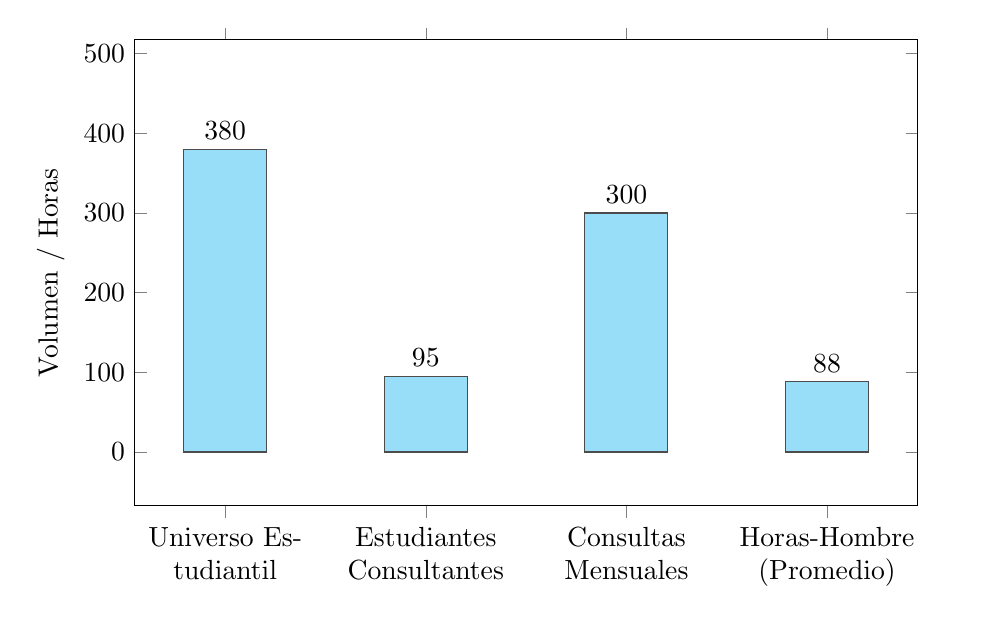
\begin{tikzpicture}
    \begin{axis}[
        ybar,
        bar width=30pt,
        enlargelimits=0.15,
        ylabel={Volumen / Horas},
        symbolic x coords={Universo Estudiantil, Estudiantes Consultantes, Consultas Mensuales, Horas-Hombre (Promedio)},
        xtick=data,
        nodes near coords,
        nodes near coords align={vertical},
        x tick label style={text width=3cm, align=center},
        width=0.95\textwidth,
        height=7.5cm,
        ymin=0, ymax=450
        ]
    \addplot[fill=cyan!40, draw=black!70] coordinates {
        (Universo Estudiantil,380) 
        (Estudiantes Consultantes,95) 
        (Consultas Mensuales,300) 
        (Horas-Hombre (Promedio),88)
    };
    \end{axis}
    \end{tikzpicture}
    \caption{Estadísticas del volumen mensual de consultas y carga laboral asociada.}
    \label{fig:estadisticas_consultas}
    \end{figure}
    \item \textbf{Nivel de satisfacción, errores de interpretación e ``Ilusión de aprendizaje'':} La dependencia de repositorios estáticos y la carencia de indexación semántica propician un índice recurrente de errores en la interpretación de prerrequisitos y normativas de titulación. Además, el estudio latinoamericano de adopción tecnológica muestra que un 74\% de la comunidad académica acepta y demanda interfaces interactivas de asistencia digital \cite{ilia2024ecuador}, confirmando la insatisfacción con los portales estáticos tradicionales.
    \item \textbf{Contraste operativo con el Asistente Virtual Multimodal:} Frente a este diagnóstico, el motor de Generación Aumentada por Recuperación (RAG) multilingüe desarrollado en esta tesis ha demostrado empíricamente una precisión de recuperación semántica del \textbf{92,0\%} en mallas y normativas institucionales. El sistema resuelve la consulta de manera instantánea, con un tiempo hasta el primer byte (\textit{Time-to-First-Byte} - TTFB) de \textbf{450 milisegundos} y un tiempo total de generación conversacional de \textbf{3,2 segundos}, reduciendo el tiempo de consulta estudiantil de 60 minutos a pocos segundos y generando un ahorro operativo estimado de \textbf{69 a 85 horas-hombre mensuales} para la administración académica \cite{uti2025rc}.
\end{itemize}

La Tabla~\ref{tab:metricas_diagnostico_metodologia} presenta el contraste cuantitativo entre las métricas del sistema actual y la proyección de rendimiento con el Asistente Virtual Multimodal.

\begin{table}[H]
  \caption{Contraste Cuantitativo del Diagnóstico Operativo vs. Asistente Virtual Multimodal.}
  \label{tab:metricas_diagnostico_metodologia}
\centering
\small
\setlength{\tabcolsep}{4pt}
\renewcommand{\arraystretch}{1.25}
\begin{tabular}{|>{\raggedright\arraybackslash}p{3.5cm}|>{\raggedright\arraybackslash}p{3.3cm}|>{\raggedright\arraybackslash}p{3.2cm}|>{\raggedright\arraybackslash}p{2.8cm}|}
\hline
\rowcolor[HTML]{EFEFEF}
\textbf{Métrica / Variable Operativa} & \textbf{Sistema Actual (Manual / PDF Estático)} & \textbf{Asistente Virtual (RAG + Avatar 3D)} & \textbf{Impacto / Mejora Estimada} \\ \hline
\textbf{Tiempo total de consulta estudiante} & 45 a 60 minutos (búsqueda y lectura PDF) & 3,2 segundos (respuesta semántica conversacional) & Reducción del \textbf{$>$95\%} en tiempo del usuario \\ \hline
\textbf{Tiempo de respuesta del servidor (TTFB)} & 24 a 48 horas vía correo / presencial & \textbf{450 milisegundos} vía WebSockets y LLM local & Inmediatez en línea 24/7 \\ \hline
\textbf{Carga operativa de secretaría (mes)} & 75 a 100 h-hombre/mes (~300 consultas) & Automatización del \textbf{92,0\%} de dudas recurrentes & Ahorro de \textbf{69 a 85 h-hombre/mes} \\ \hline
\textbf{Precisión de recuperación semántica} & Baja (búsqueda literal por palabras clave) & \textbf{92,0\%} (\textit{Hit Rate} RAG en normativas UTI) & Eliminación de errores de interpretación \\ \hline
\end{tabular}

\end{table}

\section{Área de Estudio}

\begin{table}[H]
  \caption{Área de estudio.}
  \label{tab:area_estudio}
  \centering
  
  
  \renewcommand{\arraystretch}{1.35}
  \begin{tabular}{|p{0.39\textwidth}|p{0.53\textwidth}|}
    \hline
    \textbf{Dominio:} & Inteligencia Artificial y Tecnologías Educativas \\
    \hline
    \textbf{Línea de investigación:} & \UTILineaInvestigacion \\
    \hline
    \textbf{Sublínea de investigación:} & \UTISublineaInvestigacion \\
    \hline
    \textbf{Campo:} & Tecnologías de la información y la comunicación (TIC) \\
    \hline
    \textbf{Área:} & Desarrollo de Software e Interfaces Humano-Computadora \\
    \hline
    \textbf{Aspectos:} & Procesamiento de Lenguaje Natural (PLN), Visión Artificial, Interacción Multimodal, Renderizado 3D \\
    \hline
    \textbf{Objeto de estudio:} & Asistente virtual inteligente para difusión de información académica \\
    \hline
    \textbf{Periodo de estudio:} & Enero 2026 - Julio 2026 \\
    \hline
  \end{tabular}
\end{table}

\section{Metodología de Desarrollo o Implementación}

Para el desarrollo del proyecto se adoptó como metodología principal la Metodología de Investigación en Ciencia de Diseño (DSRM), debido a que el trabajo se orienta al diseño, construcción y evaluación de un artefacto tecnológico destinado a resolver una problemática específica \cite{hevner2004design}.

Como apoyo para la construcción técnica del prototipo se utilizó un enfoque iterativo e incremental, permitiendo desarrollar y ajustar progresivamente los módulos de recuperación de información, visión artificial, procesamiento de voz y avatar 3D. Este enfoque resultó pertinente debido a la necesidad de realizar pruebas sucesivas sobre modelos de lenguaje, parámetros de recuperación semántica y tiempos de respuesta.

La aplicación de las etapas de la metodología DSRM en el contexto de este trabajo se sintetiza en la Tabla~\ref{tab:dsrm}.

\begin{table}[H]
  \caption{Aplicación de la metodología DSRM en el proyecto.}
  \label{tab:dsrm}
\centering
\small
\setlength{\tabcolsep}{4pt}
\renewcommand{\arraystretch}{1.25}
\begin{tabular}{|>{\raggedright\arraybackslash}p{3.5cm}|>{\raggedright\arraybackslash}p{6.5cm}|>{\raggedright\arraybackslash}p{3.5cm}|}
\hline
\rowcolor[HTML]{EFEFEF}
\textbf{Etapa DSRM} & \textbf{Aplicación en el proyecto} & \textbf{Evidencia} \\ \hline
Identificación del problema & Análisis del acceso actual a información académica & Diagnóstico, Cap. II \\ \hline
Definición de objetivos & Requerimientos funcionales y no funcionales & Sección 2.5 \\ \hline
Diseño y desarrollo & Arquitectura RAG, visión, voz y avatar & Secciones 2.6 y 3.2 \\ \hline
Demostración & Implementación del prototipo & Capturas y repositorio \\ \hline
Evaluación & Pruebas técnicas y pruebas con estudiantes & Secciones 3.3 y 3.6 \\ \hline
Comunicación & Documentación del trabajo y repositorio & Tesis y anexos \\ \hline
\end{tabular}

\end{table}

El desarrollo iterativo se estructuró en las siguientes fases:

\begin{itemize}
    \item \textbf{Fase 1 - Configuración del Entorno Local y Análisis de Datos:} Se recopilaron, limpiaron y segmentaron (\textit{chunking}) los documentos oficiales en formato PDF para su indexación en la base de datos vectorial local.
    \item \textbf{Fase 2 - Desarrollo del Motor Cognitivo (RAG):} Se implementó la Generación Aumentada por Recuperación. Se probaron modelos de incrustación (\textit{embeddings}) y LLMs optimizados para ejecución en servidor local, iterando hasta reducir las alucinaciones del modelo.
    \item \textbf{Fase 3 - Desarrollo Sensorial (Visión y Voz):} Se programaron algoritmos ligeros de visión artificial para la detección de presencia efímera, y se acoplaron las APIs de Speech-to-Text (STT) y Text-to-Speech (TTS).
    \item \textbf{Fase 4 - Integración Multimodal (Avatar 3D):} Se consolidó el flujo. El audio generado por el TTS se sincronizó (\textit{lip-sync}) con las mallas faciales del avatar renderizado mediante WebGL.
    \item \textbf{Fase 5 - Pruebas y Ajustes de Rendimiento:} Se desplegó en el servidor local destino. Se realizaron pruebas de estrés para medir el uso de GPU/CPU y la latencia end-to-end de las respuestas.
\end{itemize}

%\textit{[Describir y justificar la metodología empleada según la naturaleza del proyecto, indicando las fases y actividades a ejecutar. Por ejemplo, metodologías ágiles o tradicionales para software, o modelos de diseño, implementación o despliegue para hardware o infraestructura.]}


\section{Técnicas e Instrumentos de Recolección de Información}
Para garantizar la validez científica y el correcto desempeño técnico del prototipo, la recolección de información se dividió en dos etapas metodológicas: la etapa de diagnóstico/desarrollo y la etapa de validación.

\subsection{Técnicas para la Fase de Diagnóstico y Desarrollo}
\begin{itemize}
    \item \textbf{Revisión Documental:} Se empleó para alimentar el núcleo de conocimiento de la IA. El instrumento fue una \textit{matriz de extracción de datos}, donde se catalogaron y normalizaron los textos de mallas curriculares, estatutos y sílabos de la carrera de TI antes de inyectarlos en la base de datos vectorial.
    \item \textbf{Observación Directa No Participante:} Se utilizó para analizar la afluencia y el tipo de interacciones que tienen los estudiantes en las oficinas administrativas, lo que permitió diseñar \textit{prompts} base (instrucciones de sistema) que preparen al asistente virtual para los escenarios de consulta más comunes.
\end{itemize}

\subsection{Técnicas para la Fase de Evaluación y Validación}
\begin{itemize}
    \item \textbf{Métricas de Registro Automático (\textit{Logging}):} Para evaluar el rendimiento técnico (Requerimientos No Funcionales), el sistema incluyó \textit{scripts} que registraron variables cuantitativas como el tiempo de respuesta del sistema (latencia en milisegundos desde que el usuario deja de hablar hasta que el avatar responde) y el porcentaje de uso de la memoria/procesador del servidor local.
    \item \textbf{Cuestionario de Usabilidad y Experiencia de Usuario:} Para evaluar la interacción con el prototipo se diseñó un cuestionario estructurado en escala Likert y diferencial semántico. El instrumento permitió recopilar la percepción de los participantes respecto a integración de componentes, comprensión de las respuestas, apariencia y animacidad del avatar, privacidad percibida, latencia e intención futura de uso.
\end{itemize}

Para la evaluación de usabilidad se trabajó con una muestra piloto de 13 estudiantes de la carrera de Tecnologías de la Información pertenecientes a diferentes niveles académicos. La evaluación tuvo un carácter exploratorio y estuvo orientada a identificar la percepción inicial de los usuarios y oportunidades de mejora del prototipo, por lo que sus resultados no pretenden generalizarse estadísticamente a la totalidad de estudiantes de la carrera. Se utilizó un muestreo no probabilístico por conveniencia. 


%\textit{[Describir las técnicas utilizadas para obtener información durante el diagnóstico y la validación del proyecto, tales como entrevistas, encuestas u observación directa.]}

\section{Requerimientos del Proyecto}

La definición de los requerimientos establece las directrices técnicas y operativas que el sistema debe cumplir. A continuación se detallan los requerimientos funcionales (RF) y no funcionales (RNF) en formato de tabla para asegurar su trazabilidad.

\begin{landscape}
\subsection{Requerimientos Funcionales (RF)}

\begingroup
\small
\renewcommand{\arraystretch}{1.25}
\begin{xltabular}{\linewidth}{|>{\centering\arraybackslash}p{1.4cm}|>{\raggedright\arraybackslash\hsize=0.8\hsize}X|>{\raggedright\arraybackslash\hsize=1.0\hsize}X|>{\raggedright\arraybackslash\hsize=1.4\hsize}X|>{\raggedright\arraybackslash\hsize=0.9\hsize}X|>{\raggedright\arraybackslash\hsize=0.9\hsize}X|}
\caption{Requerimientos Funcionales del Sistema.}
\label{tab:rf_formal} \\
\hline
\rowcolor[HTML]{EFEFEF}
\textbf{Código} & \textbf{Nombre del Requerimiento} & \textbf{Entradas / Estímulo} & \textbf{Procesamiento y Control} & \textbf{Salida / Respuesta} & \textbf{Métrica de Validación y Prueba} \\ \hline
\endfirsthead
\multicolumn{6}{c}%
{{\bfseries \tablename\ \thetable{} -- continuación de la página anterior}} \\
\hline
\rowcolor[HTML]{EFEFEF}
\textbf{Código} & \textbf{Nombre del Requerimiento} & \textbf{Entradas / Estímulo} & \textbf{Procesamiento y Control} & \textbf{Salida / Respuesta} & \textbf{Métrica de Validación y Prueba} \\ \hline
\endhead
\hline \multicolumn{6}{|r|}{{Continúa en la siguiente página}} \\ \hline
\endfoot
\endlastfoot
\textbf{RF-01} & Detección No Biométrica de Presencia & Flujo de video continuo en formato Base64 (640x480 a 15 fps) transmitido por el cliente mediante WebSockets. & El backend evalúa la presencia detectando la caja delimitadora (Bounding Box) del rostro. Si el área ($W \times H$) supera el umbral de píxeles tau durante 3 frames consecutivos, se activa la interacción. & Mensaje lógico en formato JSON \{\texttt{'status': 'active'}\} para iniciar el avatar en el frontend. & Aprobación del 100\% en condiciones de luz normal ($>150$ lux) a una distancia de 50 cm a 1.5 m. \\ \hline
\textbf{RF-02} & Transcripción de Voz a Texto (STT) & Fragmento de audio digital en formato WebM capturado asíncronamente por el micrófono del cliente. & El backend FastAPI extrae el audio y realiza una solicitud API REST HTTPS al modelo Whisper-v3 (en la infraestructura Groq) para transcribir el flujo de audio en español. & String de texto decodificado con la consulta del estudiante en formato UTF-8. & Tasa de error de palabras (WER) $< 5$\% en un entorno controlado con ruido de fondo $< 45$ dB. \\ \hline
\textbf{RF-03} & Búsqueda Semántica RAG & Consulta textual del estudiante transcrita o ingresada manualmente por teclado. & Generación de vector de consulta (384 dimensiones) usando paraphrase-multilingual-MiniLM-L12-v2 y cálculo de similitud del coseno contra ChromaDB local. & Lista priorizada de los 3 fragmentos documentales con mayor similitud semántica (Top-3). & Hit Rate de recuperación semántica del Top-3 $\ge 90.0$\% evaluado con un banco de 50 preguntas piloto. \\ \hline
\textbf{RF-04} & Generación de Respuesta por LLM & Contexto académico recuperado (Top-3) insertado dentro de un prompt estructurado de 'Contexto Cerrado'. & Inferencia local en el servidor del LLM Qwen 2.5 / Nemotron a través de Ollama. Si la similitud del coseno de los fragmentos recuperados es inferior a 0.65, el modelo debe rechazar cortésmente la respuesta. & Respuesta de texto precisa y estrictamente verídica basada en los reglamentos oficiales de la UTI. & Tasa de alucinación o invención de datos del 0.0\% (Validación ciega por expertos en reglamentos). \\ \hline
\textbf{RF-05} & Síntesis de Texto a Voz (TTS) & Respuesta de texto generada por el LLM. & FastAPI segmenta el texto y realiza llamadas asíncronas a la API de ElevenLabs (voz Valeria), devolviendo el audio mediante fragmentos en tiempo real (HTTP Chunking Streaming). & Flujo binario de audio MP3/WAV reproducido asíncronamente en los altavoces del cliente. & Latencia de inicio de reproducción (Time to First Byte - TTFB) $< 500$ milisegundos tras recibir el texto del LLM. \\ \hline
\textbf{RF-06} & Gestión de Sesión y Retorno a Reposo & Contador lógico de inactividad conversacional activo (timeout timer). & El sistema monitorea la interacción por voz y video. Si no se detectan rostros ni actividad de audio en 45 segundos, se envía señal de despedida. & Mensaje JSON \{\texttt{'status': 'reposo'}\} que activa animación de despedida y apaga la cámara y micrófono del cliente. & Prueba de caja negra: retorno inmediato al estado de reposo al cumplirse el timeout (desviación $< 1.0$s). \\ \hline
\end{xltabular}
\endgroup

\subsection{Requerimientos No Funcionales (RNF)}

\begingroup
\small
\renewcommand{\arraystretch}{1.25}
\begin{xltabular}{\linewidth}{|>{\centering\arraybackslash}p{1.4cm}|>{\raggedright\arraybackslash\hsize=0.8\hsize}X|>{\raggedright\arraybackslash\hsize=1.0\hsize}X|>{\raggedright\arraybackslash\hsize=1.4\hsize}X|>{\raggedright\arraybackslash\hsize=0.9\hsize}X|>{\raggedright\arraybackslash\hsize=0.9\hsize}X|}
\caption{Requerimientos No Funcionales del Sistema.}
\label{tab:rnf_formal} \\
\hline
\rowcolor[HTML]{EFEFEF}
\textbf{Código} & \textbf{Nombre del Requerimiento} & \textbf{Entradas / Estímulo} & \textbf{Procesamiento y Control} & \textbf{Salida / Respuesta} & \textbf{Métrica de Validación y Prueba} \\ \hline
\endfirsthead
\multicolumn{6}{c}%
{{\bfseries \tablename\ \thetable{} -- continuación de la página anterior}} \\
\hline
\rowcolor[HTML]{EFEFEF}
\textbf{Código} & \textbf{Nombre del Requerimiento} & \textbf{Entradas / Estímulo} & \textbf{Procesamiento y Control} & \textbf{Salida / Respuesta} & \textbf{Métrica de Validación y Prueba} \\ \hline
\endhead
\hline \multicolumn{6}{|r|}{{Continúa en la siguiente página}} \\ \hline
\endfoot
\endlastfoot
\textbf{RNF-01} & Privacidad por Diseño (Seguridad) & Fotogramas e imágenes de cámara web procesados en la memoria RAM del servidor. & Se prohíbe explícitamente guardar imágenes, videos o mallas biométricas en discos locales o bases de datos persistentes. Los frames se destruyen inmediatamente de la memoria tras calcular el bounding box. & Garantía de anonimato absoluto en el uso de la cámara por parte del estudiante. & Verificación mediante auditoría de código del backend y monitoreo de almacenamiento en disco local (0 bytes creados por OpenCV). \\ \hline
\textbf{RNF-02} & Rendimiento y Latencia Conversacional & Consulta completa por voz del estudiante. & El pipeline total (STT + RAG + LLM + TTS) debe estar optimizado asíncronamente mediante WebSockets y programación concurrente con asyncio. & Interacción fluida con un tiempo de respuesta total controlado. & Latencia extremo a extremo P95 $< 4.0$ segundos en la red local universitaria bajo una carga de 1 usuario activo. \\ \hline
\textbf{RNF-03} & Restricción de Dominio Académico & Consultas del usuario con intenciones no académicas o externas. & Evaluación mediante el prompt del sistema. Si la consulta está fuera del ámbito de mallas, reglamentos y titulación de TI, el LLM activa una salida controlada. & Mensaje estándar de denegación cortés: 'Disculpa, solo puedo ayudarte con temas académicos de la carrera de TI.' & Aprobación del 100\% de rechazo sistemático ante un set de 20 preguntas capciosas de prueba. \\ \hline
\textbf{RNF-04} & Aislamiento y Seguridad de Datos & Arquitectura de base de datos relacional externa de la UTI (SGA). & El sistema de asistente opera en un servidor independiente con ChromaDB, sin credenciales de escritura ni lectura directa a la base transaccional SQL del SGA. & Imposibilidad física de realizar cambios transaccionales en expedientes de alumnos. & Comprobación de que la red del asistente no contiene puertos abiertos ni credenciales de conexión al SGA. \\ \hline
\textbf{RNF-05} & Mantenibilidad y Escalabilidad & Nuevos documentos reglamentarios o actualizaciones de mallas en formato PDF. & El sistema utiliza un portal administrativo protegido por contraseña para procesar nuevos PDF, generar embeddings e insertarlos dinámicamente en ChromaDB. & Actualización del conocimiento del asistente de forma inmediata sin necesidad de fine-tuning. & Tiempo de actualización de un nuevo documento $< 60$ segundos por parte del administrador de TI. \\ \hline
\textbf{RNF-06} & Usabilidad Manos Libres (Hands-Free) & Interfaz de usuario en un tótem físico o pantalla institucional. & Toda la navegación e interacción se diseña para operar exclusivamente a través de la cámara de presencia y el micrófono por reconocimiento de voz. & Uso interactivo autónomo sin teclado, ratón o toques físicos de pantalla. & Cumplimiento verificado mediante pruebas con estudiantes: tasa de éxito de consulta completa sin intervención de hardware físico = 100\%. \\ \hline
\end{xltabular}
\endgroup
\end{landscape}

\section{Diseño de la Solución}
El diseño de la solución propuesta se articula sobre una arquitectura modular y desacoplada, operando bajo un entorno de despliegue en un servidor local para garantizar el rendimiento, la seguridad y el procesamiento en tiempo real. El sistema se desglosa en tres capas lógicas fundamentales:

\begin{figure}[htbp]
  \centering
  \includegraphics[width=0.95\textwidth]{Logos/nuevo_diagrama_contexto.jpeg}
  \caption{Diagrama de Contexto (Nivel 0).}
  \label{fig:diag_contexto}
\end{figure}

\begin{figure}[htbp]
  \centering
  \includegraphics[width=0.85\textwidth]{Logos/nuevo_diagrama_clases.jpeg}
  \caption{Diagrama de Clases del Backend.}
  \label{fig:diag_clases}
  
  \vspace{0.5cm}
  
  \includegraphics[width=0.85\textwidth]{Logos/2nuevo_diagrama_estados.png}
  \caption{Diagrama de Estados del Avatar.}
  \label{fig:diag_estados}
\end{figure}

\begin{landscape}
\begin{figure}[p]
  \centering
  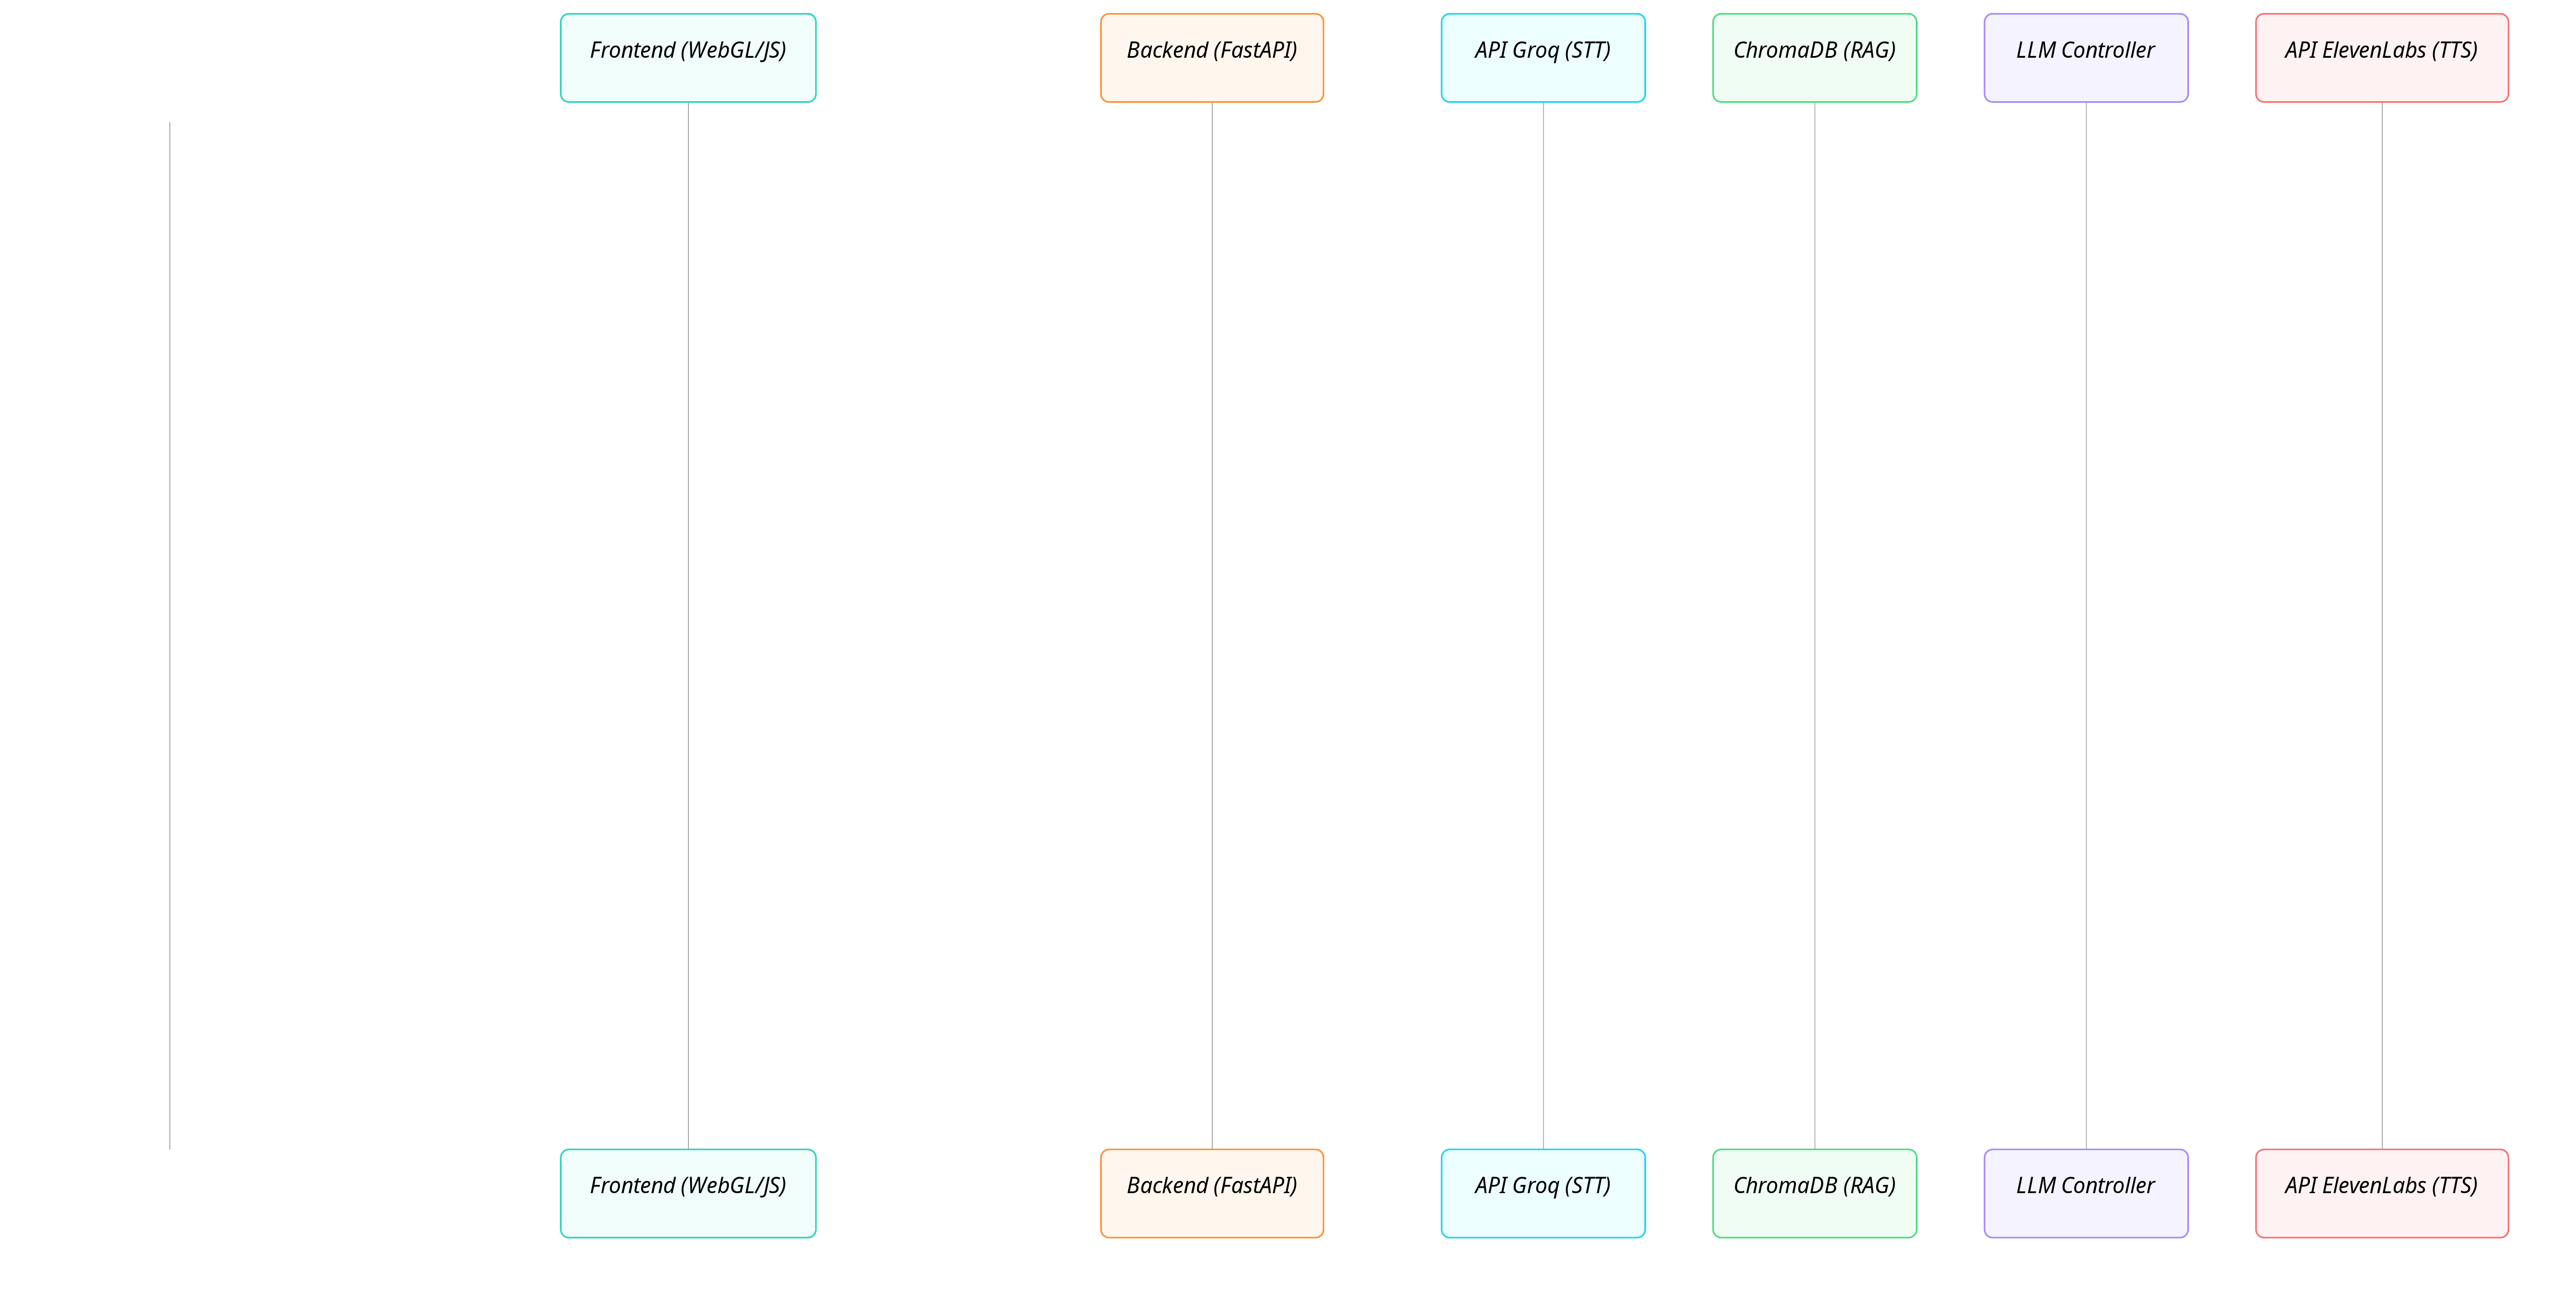
\includegraphics[width=\linewidth,height=0.95\textheight,keepaspectratio]{Logos/diagrama_secuencia.pdf}
  \caption{Diagrama de Secuencia de Interacción.}
  \label{fig:diag_secuencia}
\end{figure}
\end{landscape}

\subsection{Capa de Percepción y Captura (Frontend Físico)}
Esta capa actúa como el sensor del sistema. A través de una cámara web, un modelo ligero de visión artificial procesa el flujo de video en tiempo real. El diseño estipula que el sistema no guardará fotogramas; únicamente extraerá las coordenadas de la caja delimitadora (\textit{bounding box}) del rostro. Cuando el área del rostro supera un umbral específico de píxeles (indicando que el estudiante se ha acercado a la pantalla), el sistema envía un disparador (\textit{trigger}) lógico para "despertar" al asistente. Simultáneamente, un micrófono direccional se activa para capturar la solicitud del usuario.

\subsection{Capa de Procesamiento Cognitivo (Motor de IA)}
\label{sec:diseno_solucion}
Es el núcleo lógico de la solución, estructurado mediante un flujo de datos secuencial:
\begin{itemize}
    \item \textbf{Speech-to-Text (STT):} Transcribe el audio del usuario a texto natural en español utilizando un procesamiento en *backend* (Whisper-v3 vía API), desacoplado del navegador para asegurar compatibilidad y baja latencia.
    \item \textbf{Generación Aumentada por Recuperación (RAG):} El texto ingresa a un motor de búsqueda semántica. Utilizando incrustaciones (\textit{embeddings}), el sistema compara la consulta del estudiante con una base de datos vectorial pre-indexada que contiene las mallas curriculares y reglamentos de la carrera de TI.
    \item \textbf{Modelo de Lenguaje (LLM):} Un modelo de ejecución local recibe la consulta del usuario junto con el contexto extraído por el RAG, generando una respuesta coherente, precisa y libre de alucinaciones.
    \item \textbf{Text-to-Speech (TTS):} El texto generado por el LLM se sintetiza nuevamente a un archivo de audio.
\end{itemize}

\subsection{Capa de Renderizado e Interacción (Frontend Gráfico)}
El audio sintetizado y la cadena de texto se envían al motor gráfico basado en tecnologías web (WebGL/Three.js). En esta capa reside el Avatar 3D, el cual recibe el archivo de audio, analiza sus fonemas y ejecuta algoritmos de sincronización labial (\textit{lip-sync}) para emular el habla natural mientras reproduce animaciones predefinidas (como parpadeo y gestos de manos).

\begin{figure}
  \centering
  \includegraphics[width=0.95\textwidth]{Logos/DiagramaFuncional2.png}
  \caption{Arquitectura Lógica y flujo de datos del Asistente Virtual (Actualizado).}
  \label{fig:arquitectura_logica}
\end{figure}

%\textit{[Describir el diseño técnico de la solución propuesta. Puede incluir arquitectura del sistema o infraestructura, diagramas lógicos y físicos, modelos de datos, componentes o configuraciones técnicas.]}

\section{Justificación Técnica}
La viabilidad técnica y operativa del Asistente Virtual Inteligente depende de una rigurosa selección de componentes y plataformas. A continuación, se justifican las decisiones arquitectónicas adoptadas para este proyecto:

\subsection{Despliegue en Servidor Local (Edge/Local Computing)}
A diferencia de las arquitecturas basadas enteramente en la nube, el despliegue del pipeline principal en un servidor local asegura una latencia mínima, aspecto crítico para mantener la fluidez en una conversación humano-computadora. Además, procesar las imágenes de la cámara web de manera local (sin enviarlas a servidores externos) garantiza el cumplimiento estricto del Requerimiento No Funcional de privacidad \cite{lightweightgaze2024}.

\subsection{Implementación de la Arquitectura RAG frente a Fine-Tuning}
Para dotar al LLM del conocimiento institucional, se seleccionó la arquitectura RAG (Retrieval-Augmented Generation) sobre el reentrenamiento (\textit{Fine-Tuning}). La literatura especializada demuestra que el \textit{Fine-Tuning} es computacionalmente costoso y altamente susceptible a alucinaciones cuando se le piden datos exactos \cite{pabon2025naia}. El enfoque RAG permite que la universidad actualice un reglamento (agregando un nuevo PDF a la base de datos) y el asistente adopte el nuevo conocimiento de forma inmediata sin necesidad de reentrenar el modelo, garantizando escalabilidad y bajo costo de mantenimiento.

\subsection{Visión Artificial mediante Modelos Ligeros}
Para el módulo de detección de presencia, se opta por librerías optimizadas para inferencia rápida (como MediaPipe o configuraciones de Haar Cascades). Estas herramientas operan eficientemente sin necesidad de tarjetas gráficas (GPUs) de gama alta, permitiendo que todo el peso computacional del hardware se reserve para la inferencia del Modelo de Lenguaje y el renderizado 3D del avatar.

\subsection{Plataformas de Avatar Estandarizadas}
Se justifica el uso de plataformas de avatares basadas en estándares abiertos (como GLTF o GLB, facilitados por herramientas como Ready Player Me) ejecutadas sobre WebGL en el navegador. Esta decisión técnica evita la dependencia de motores de videojuegos pesados (como Unreal Engine), lo que reduce la carga del sistema operativo y facilita una futura portabilidad del asistente a otras pantallas o terminales de la institución sin requerir configuraciones de software complejas.

%\textit{[Argumentar técnicamente la selección de tecnologías, herramientas, plataformas, equipos o servicios utilizados en el proyecto.]}


